\Chapter{EMAIL2GIT: FROM ACADEMIC RESEARCH TO OPEN-SOURCE SOFTWARE}\label{sec:Theme2}

As explained in \autoref{sec:Introduction}, the linux contribution process is a strong email-based system that has proven to be more reliable and scalable over the years. Like in many other organizations, the linux development community makes extensive use of code reviews to ensure the quality of contributors' code submissions. These code reviews occur in the mailing lists, where the patch was first introduced. After accepting and integrating the patch to the git repository, it is usually very hard to recover the original patch, the code reviews, and the discussion that took place during the code reviews. 

Other tools have addressed this issue by providing a code review environment and by keeping track of the code review for each commit. However, these environments often do not broadcast the code reviews to everyone. These \textit{unicast} review environment only allow the author to read the code reviews. In a quantitative study, \citep{armstrong} examined the differences between \textit{unicast} and \textit{broadcast} review system. The authors discovered that broadcast allows for faster review cycle, and provides learning material for new developers. The linux community never used these tool for upstream contributions as they would not scale to the size of the linux community. 


To address the lack of way to backtrack reviews, we implemented Email2git. The tool is able to find, for a given linux commit, the orignal patches and the code reviews. This chapter introduce Email2git, from its inception, to its deployement to production. 

\section{Previous Publications and Original Algorithm}

The original algorithm capable of backtracking patches from commits was introduced in two papers~\citep{msr13jojo,jiang14} published by Jiang, a former member of the MCIS Lab. The general idea of the algorithm was to compare the +/- lines from both the git commits and the email patches. A match was found if the proportion of identical +/- lines was above a certain threshold. Although this script was a great proof of concept, it had difficulties scalling to 8 years of emails and commits. 



\section{Scalling the Algorithm}

Because we wanted Email2git to be a usable and practical tool, we needed a way to display the patches and the code reviews in a browser. Fortunatly, an existing open-source tool called \textbf{Patchwork}\footnote{\url{https://github.com/getpatchwork/patchwork}} perfectly answers our requirements. Patchwork is a tool designed to assist maintainers of open source projects using an email-based contribution process. It tracks the mailing lists used by developers to submit patches and recieve code reviews. The tool extracts each detected patch as well as its associated reviews, then displays them in a web-based user interface. 

We were granted read access to the MySQL database behind a patchwork instance hosted on kernel.org\footnote{\url{https://patchwork.kernel.org/}}. This instance has been tracking 69 of the many linux subsystems mailing lists since 2009, giving us the oportunity to analyse over \textit{1.4 million} patches.

In addition to being a data source, patchwork.kernel.org also represents a way for us to display the patches and the code reviews associated with commits to the users. The only limitation of this patchwork instance is that it does not track some major mailing lists, particularly some of the \texttt{Net} mailing lists. 


Since we had access to email patches dating back to 2009, we decided to extract git commits from the Linux git repository from the same date, which represent over \textit{500,000 commits} to analyse. Unfortunatly, this amount of data was too large for the orignal algorithm to parse in a timely fashion, which called for a new, scalable algorithm that leverages heuristics mentioned in \citep{msr13jojo,jiang14}.

\subsection{Patch Email Subject}

The most important heuristic that drastically increased the matching speed is the \textit{email subject - commit summary} concept. The built-in git features \texttt{git format-patch} and \texttt{git send-email} allows developers to easily submit their changes to a maintainer by email according to the Linux Kernel Contribution guidelines\footnote{\url{https://kernelnewbies.org/FirstKernelPatch}}. This or these emails contain all the meta-data that will eventually be included in the commit, if the patch is accepted. The meta-data includes heuristics such as: time sent, author, commit message, ... If the patch is accepted, the maintainer can use another git command to integrate the patch into her repository: \texttt{git am}\footnote{\url{https://git-scm.com/docs/git-am}}. This command will automatically exctract the patch info and keep the relevant information in the commit. The piece of information we are interested in is the email subject. \texttt{Git am} automatically saves the email subject and uses it the "commit summary". This commit summary, or commit title, is the first line of the commit message (((TODO: refer to intro for git commit stuff))). Comparing both strings of characters allows for a very quick first phase of matching.

This first phase will find a match for about 55\% of the commits. After this step, we can remove the commits and the patches that were matches from the "search space", reducing the amount of patches and commits to be parsed, reducing the load on the algorithm. 

\subsection{Author and Affected Files}

Even though the number of commits was reduced by half after the first phase, I was unable to make the old script fast enough to parse the rest of the data in a timely fashion. Thus, I had to find a way to use the available meta-data to speed up the matching. The first data point I used was the \textit{author name}. As depicted in \autoref{fig:author_matching}\alex{TODO: Improve schema}\alex{Not sure how technical I should get}, I am able to use the name and email address of the \textit{commit author} to pin point to the patches that were sent by the same person. In other words, to find a match for each commit, the algorithm has to parse a handfull of patches instead of hundreds of thousand. Similarly, the files affected by a commit and a patch can drasticaly help the performance of the +/- line algorithm. Through some regular expression and text parsing, we can retrieve the files that are modified in the patch and the \textit{commit diff}. Since the author-based matching is slighty faster and returns more matches than the file-based matching, we start with the former, removing each matched commit and patch to reduce the workload of the next phase.

In this phase as well as the next one, the matches are found using the same +/- lines as the original algorithm, which is a fairly slow process, although this process could be improved using a hashing-based method to find corresponding +/- lines for further performance improvement. 



\begin{figure}[htb]
\centering
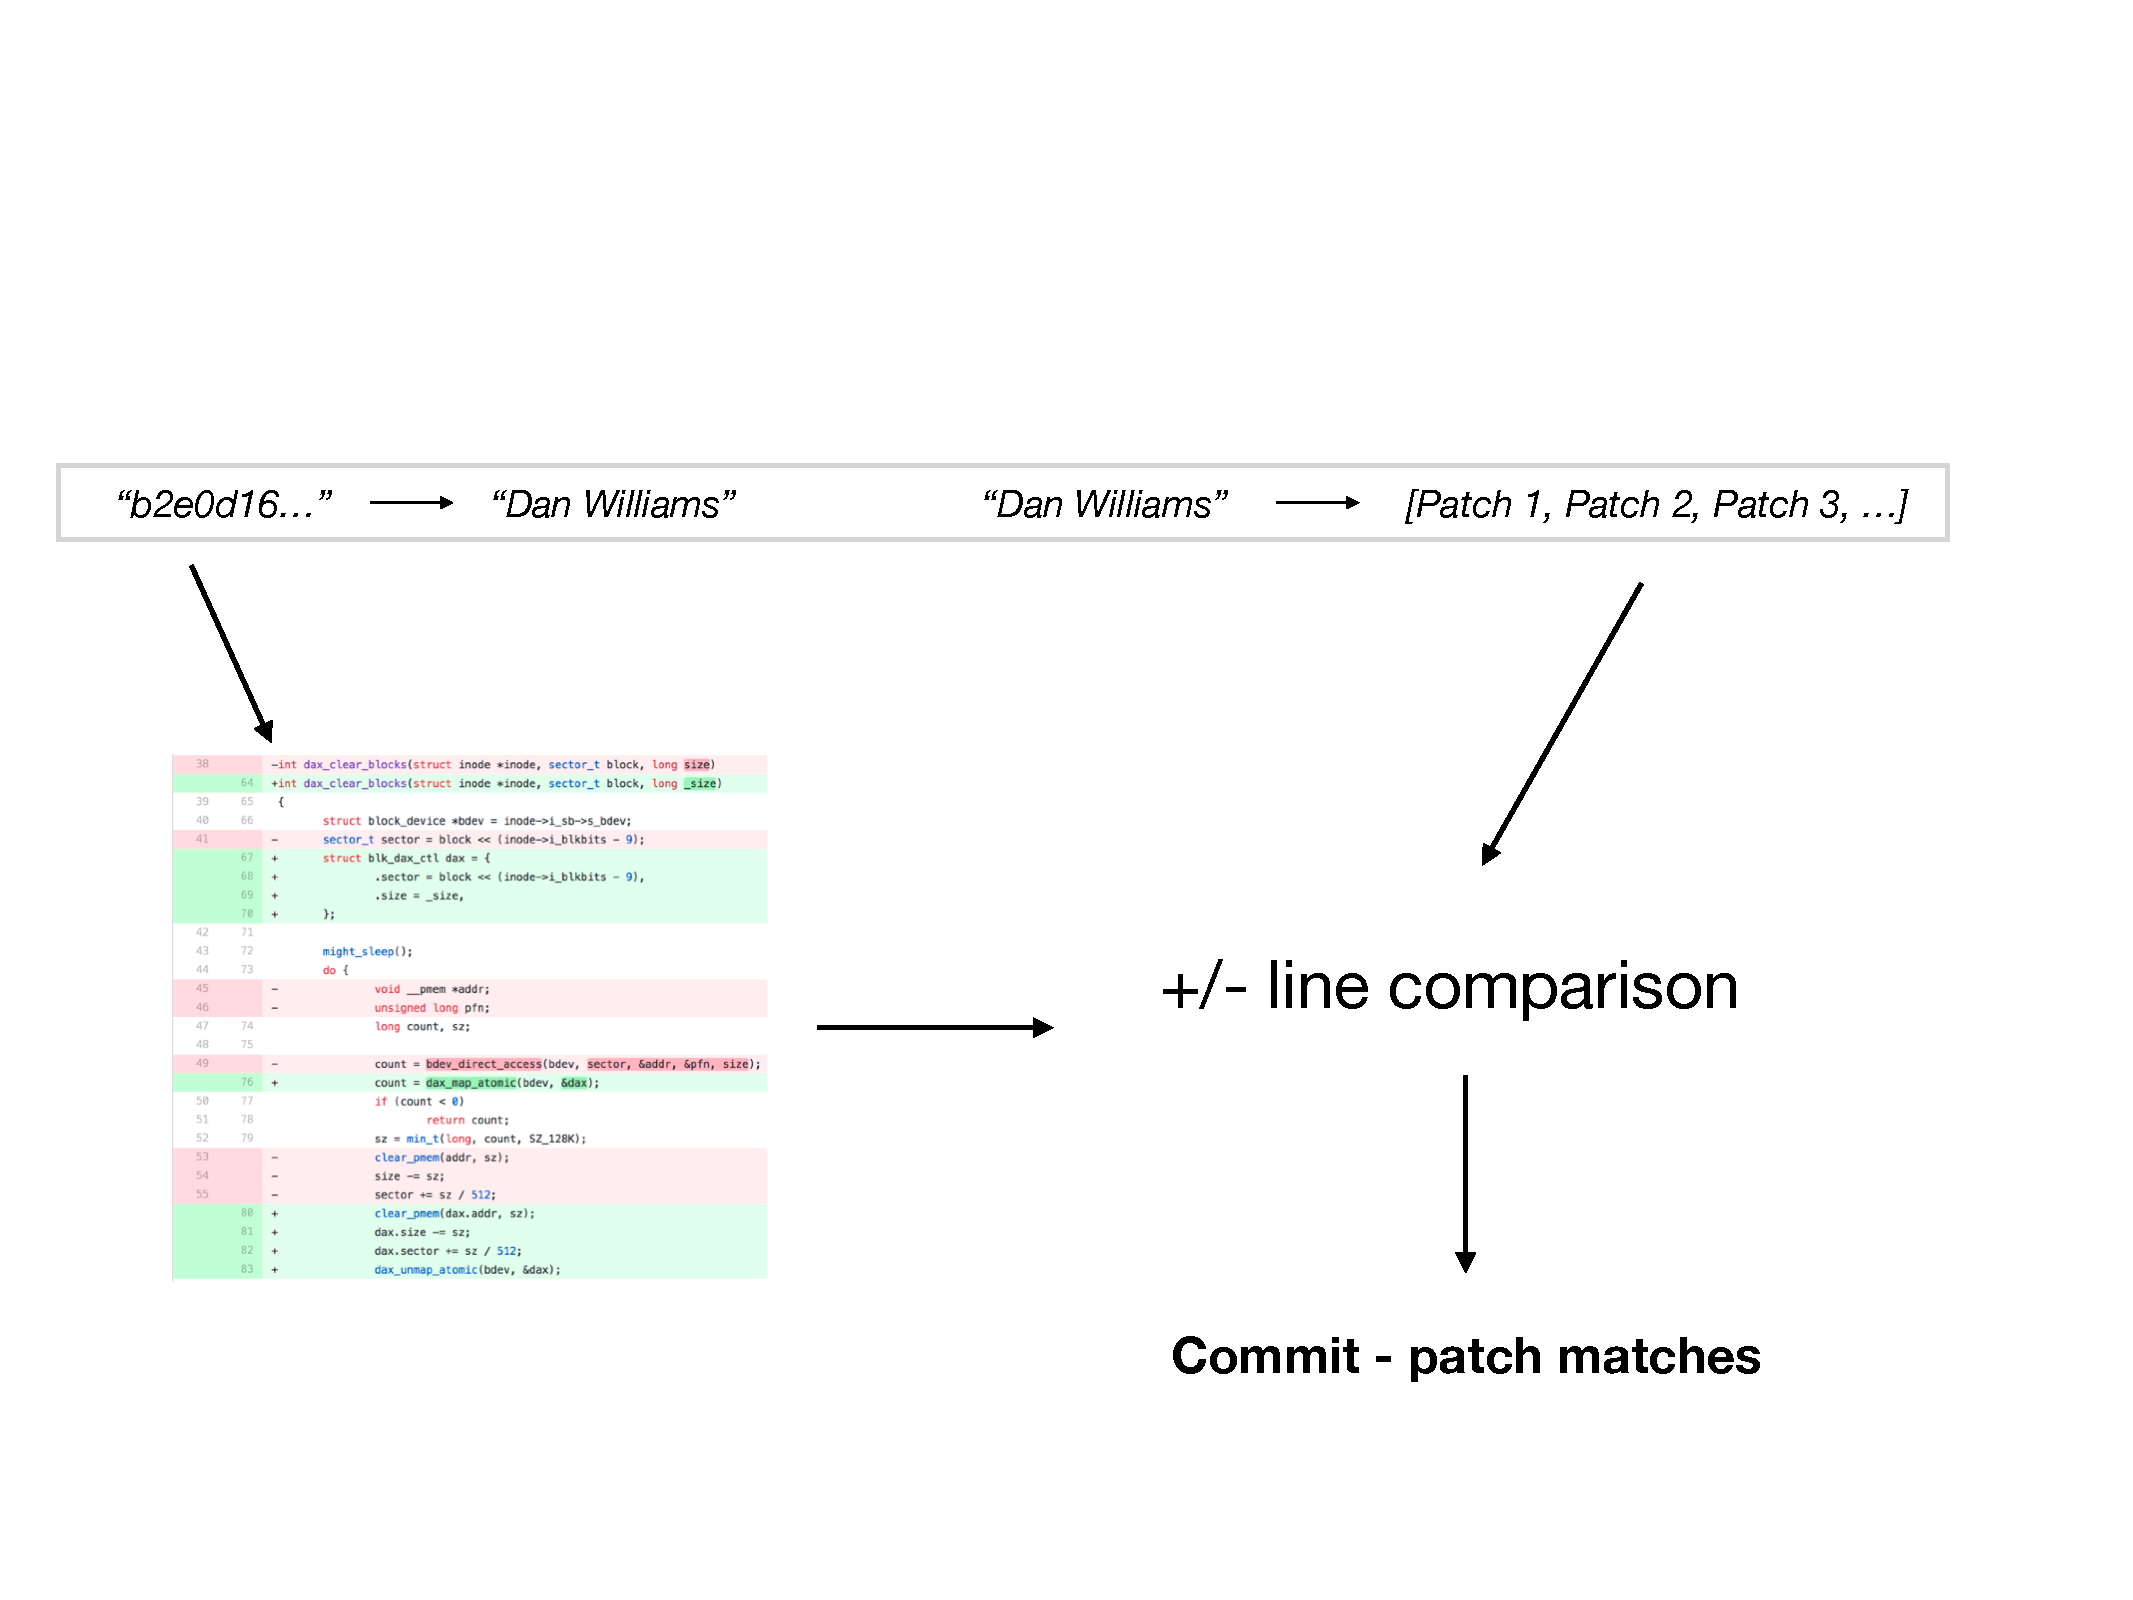
\includegraphics[width=5in]{author_matching}
\caption{Using the patch sender to assist matching}
\label{fig:author_matching}
\end{figure}


\section{The Data}

There are two sides to this matching process: the Linux git repository and the archives containing the patches sent in mailing lists over the years. We need to extract the diff (+/- lines), the metadata, and the subject and commit summary from both side. The scripts used for each part of the data extraction are available on the project's github under the GPL-3.0 license \footnote{\url{https://github.com/alexcourouble/email2git}}.



\subsection{The Commits}

First, we need to extract the commit summary from each commit after 2009. This date is our lower bound because our email data from patchwork.kernel.org only has email patches dating back to 2009. The commit summary is the first line of the commit message, which makes it very easy to retrieve. The script \texttt{subject\_data\_gen/commit\_subject\_generator.py} reads a git log output and stores the commit summary for each commit in a SQLite3 database. The exact git log command used is the following:
\begin{lstlisting}
git log --no-merges --pretty=format:"%H,%ct,%s" --after={2009-01-01}
\end{lstlisting}
The \texttt{pretty} option formats the output according to the passed parameters. 

The next step on this side of the data is to extract the data for the other phases of the matching process. The script \texttt{lines\_data\_prep/git\_prep.py} is more complicated, as there is more data to parse and save. This script reads the authors and the files affected by each commit. It will then create two maps: commit ID to author, and commit ID to files affected. These maps, which exist as python dictionaries are then saved to two separate pickle files\footnote{\url{https://docs.python.org/2/library/pickle.html}}, which make writting, reading, and storing data a fast and easy. This script also extracts the +/- lines from the commit diff and stores them in a pickle file as well. 



\subsection{The Patches}

The patches are stored on a remote serve in a MySQL database, the same database that hosts the patchwork.kernel.org data. Through the help of SQL queries, I dumped all the necessary data in csv files to avoid complications arising from handling a production database. Once those csv files created, I could parse them with the help of two python scripts available in the Email2git githubg repository. \texttt{subject\_data\_gen/patchwork/pwSubjectFull.py} takes care of the subject data and \texttt{lines\_data\_prep/pw\_prep.py} takes care of the authors, file names, and +/- lines of the patches. Here again, the subject data is stored in a SQLite3 database, and the line data is stored in pickle files. 







\section{Providing Access to the Matches}

Email2git's original inteded contribution was to increase the amount of information existing around a commit by providing access to the conversation that took place during the creation of the patch. And now that matches have been generated and saved, we need a way to make the information available to linux developers. Each match is composed of four elements: the \textit{commit ID}, the \textit{patchwork permalink ID}, the \textit{date}, and the \textit{phase} that found the match (subject, author, or file). The patchwork permalink ID is used to point to the patch and conversation on patchwork.kernel.org.

As discussed in chapter 3, the matches are available through two platforms: cregit and as a standalone commit lookup page. And although both platforms use the same UI and fetching mechanism to display the links to patchwork, the user experience is fundamentally different. On cregit, users navigate the interface by browsing the tokenized files. Once the user clicks on a token, we display a window containing the links to the patches and converstation that introduced that token to the source code. Note that in this case, the user need not to know the commit ID of of the token of interest. The commit ID, which is necessary to retrieve the patches, is hard-coded in the html element containing the token. The HTML element containing a token looks like this:

\begin{lstlisting}[language=HTML]
<a onclick="return 
windowpopLinux('2ebda74fd6c9d3fc3b9f0234fc519795e23025a5')">
	include
</a>
\end{lstlisting}

The onclick event calls a function defined in a global javascript file: \texttt{cregit.js}. In the original implementation of the cregit interface, this function would open a new browser window and show the commit associated by the token on github. So I modifed \texttt{cregit.js} to disable the "popup mechanism" and to instead use the commit ID to fetch the patchwork permalinks IDs from the server. The matches are stored as csv files named after the commit ID they are associated with on the server hosting the interface. The assyncronous requested is done throught Papaparse\footnote{\url{http://papaparse.com/}}, a powerful opensource javascript library capable of downloading and parsing csv files from the client. The javascript code that generate the URLs from the permalinks and displays the new window lives in a callback function that executes after the request is complete. We were able to keep the "view commit on github" feature, by showing a button in the new window.  

On the standalone commit ID lookup page, the mechanism is almost identical, but the user experience is completely different. Instead of clicking on a token, the user knows the commit ID in advance, as they might have encountered it while trying to fix a bug, or read a \texttt{git log} output. The user copies and pastes the commit ID in the search bar, and the match window appears with a list of dated links to patchwork. The lookup page verifies whether the commit ID is a SHA-1 hash with the following regex:

\begin{lstlisting}
// removing white space
cid = cid.replace(/\s/g, '');

// validating input
if (!/\b[0-9a-f]{40,40}\b/.test(cid)){
    window.alert("The input should be a full 40-character SHA1 hash.");
    return;
}
\end{lstlisting}

We are running analytics on the server hosting the matches to understand the usage of the data and to know the proportion of requested commit IDs are not matched. Removing the whitespace and assuring the validity of the string ensures the accuracy of these statistics, by recuding the number of failed requests due to a poorly formated commit ID.

 \begin{figure}[htb]
\centering
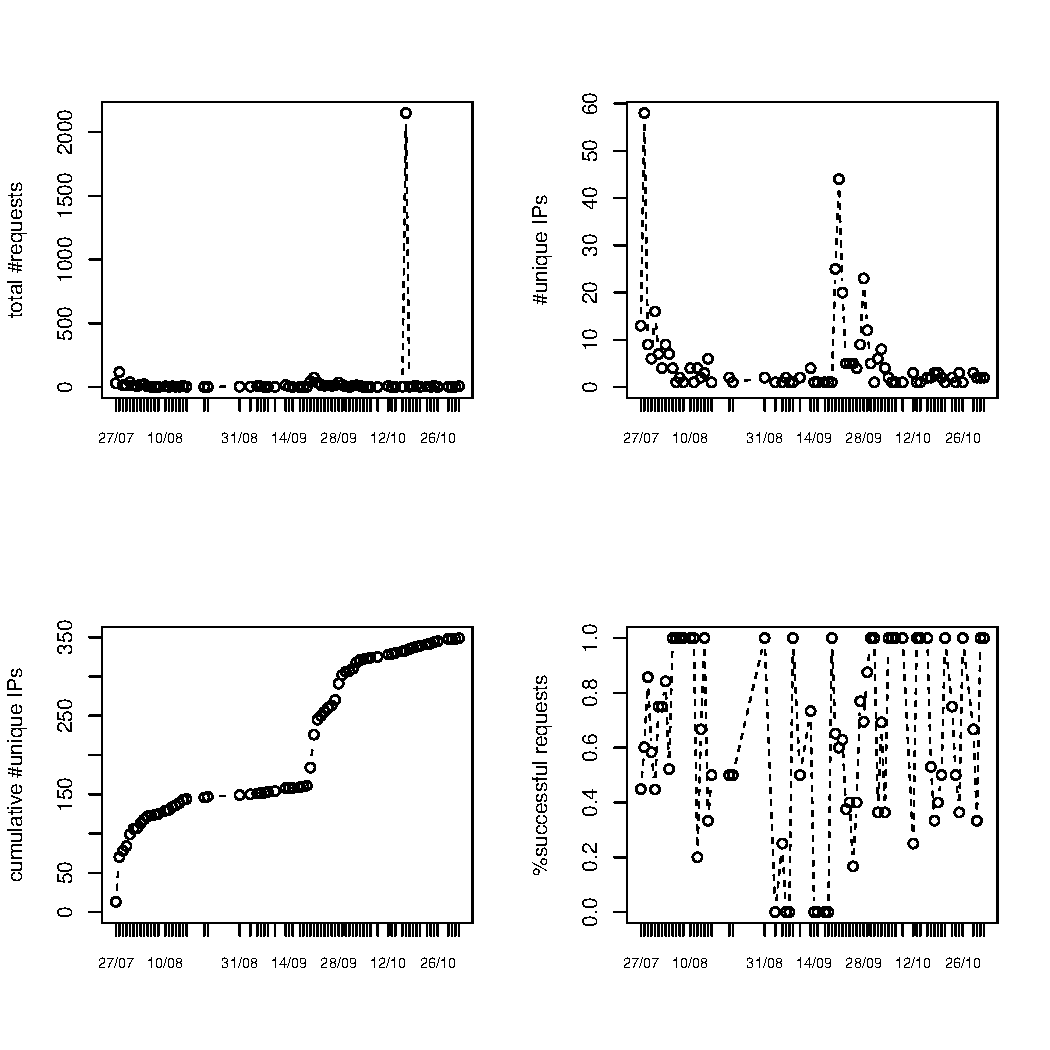
\includegraphics[width=5in]{analytics}
\caption{Plots created from the analytic}
\label{fig:analytics}
\end{figure}

\autoref{fig:analytics} displays the plots created by the analytics script running on the server. We observe two peaks in number of unique IP addresses at two different moments: at the end of July and in mid September. The former date corresponds to the day we introduced Email2git in a blogpost on linux.com and the latter corresponds to the talk I gave at the Open Source Summit North America in Los Angeles. 



\section{Introducing Email2git to the Opensource Community}

We undertook various efforts to make our work more visible to the linux and open source community in general. The first effort was a blog post published on linux.com\footnote{\url{https://www.linux.com/blog/email2git-matching-linux-code-its-mailing-list-discussions}}. This blog post discusses email2git and its integration with cregit. This blog post was shared on Facebook and Twiter by the Linux Foundation and by other developers, which helped spreading the word about our work. In addition to this blogpost, I gave a refereed talk at the Open Source Summit and the Linux Plumbers Conference in Los Angeles. This gave me the oportunity to give a demo, explain the underlying algorithm and finally discuss the project with developer and recieve crucial feedback. An article\footnote{\url{https://lwn.net/Articles/734018/}} was published on LWN.net by Jake Edge following my talk. It explained the algorithm, the chalenges faced, and mentioned some of the questions the were asked during the talk.




\alex{Should I nclude the entire blogpost? As an annex?}



